\documentclass[a4paper,12pt]{article}
\usepackage[utf8]{ inputenc}
\usepackage[ngerman]{babel}
\usepackage[a4paper, left=2.5cm, right=2.5cm]{geometry}
\usepackage{graphicx}
\usepackage{subcaption}
\usepackage{fancyhdr}
\usepackage{pdfpages}
\usepackage{listings}
\usepackage{hyperref}
\usepackage[official]{eurosym}
\usepackage{float}

\pagestyle{fancy}
\lstset{
	language=Matlab,
	breaklines=true,
	morekeywords={matlab2tikz},
	keywordstyle=\color{blue},
	morekeywords=[2]{1}, keywordstyle=[2]{\color{black}},
	identifierstyle=\color{black},
	stringstyle=\color{mylilas},
	commentstyle=\color{mygreen},
	showstringspaces=false,
	mathescape=true
	emph=[1]{for,end,break},emphstyle=[1]\color{red},
}

\hypersetup{
	colorlinks=true,
	linkcolor=blue,
	filecolor=magenta,      
	urlcolor=cyan
}

\lhead{Standort von Windkraftanlagen}
\chead{}
\rhead{Gruppe D}

\begin{document}
	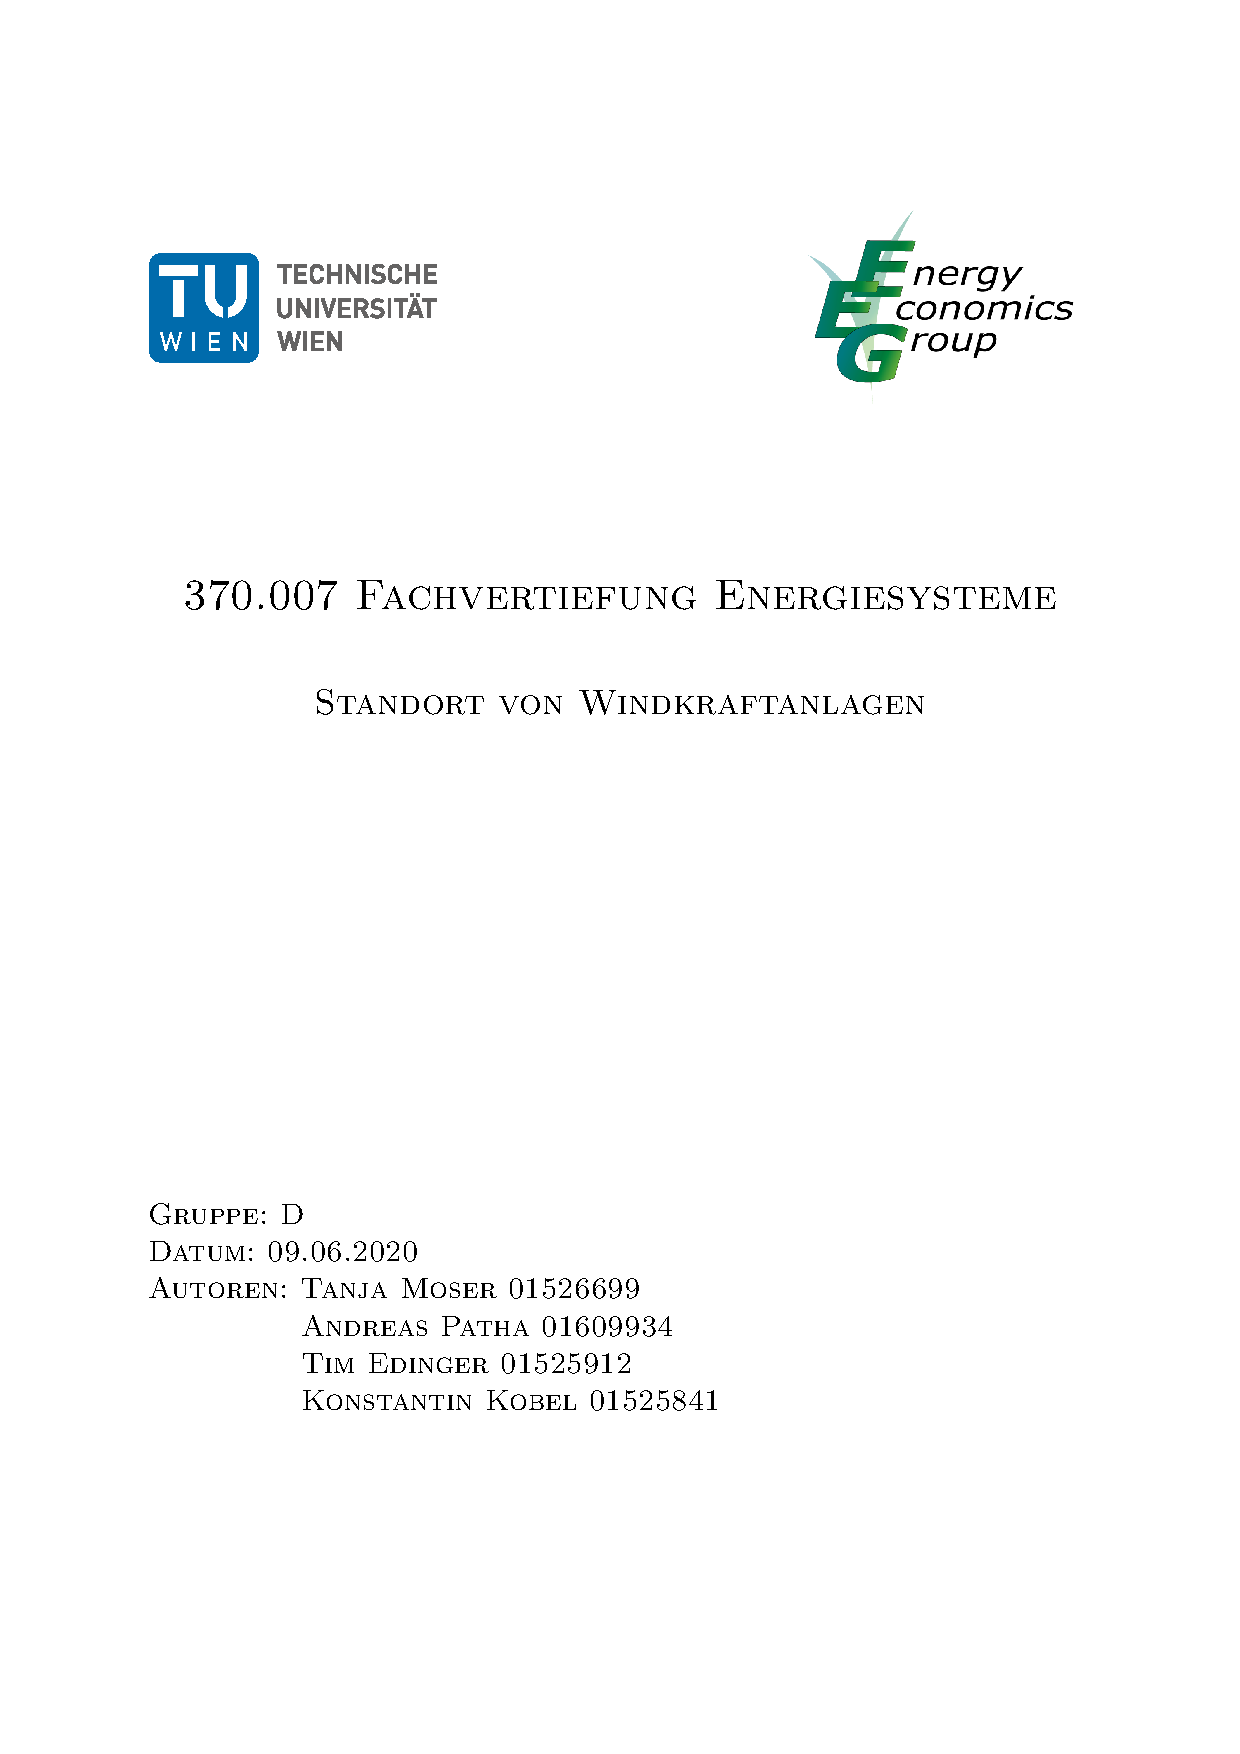
\includepdf{Protokoll_titlepage.pdf}

	\newpage
	\tableofcontents

	\newpage
	
	\section{Konzept}
	Für die 5. Abgabe möchten wir unterschiedlichen Standorte von Windkraftanlagen miteinander vergleichen.\\ \par
	\noindent Im Speziellen sollen zwei Aspekte mit einander verglichen werden:
	\begin{itemize}
		\item Offshore vs. Onshore
		\item Standort in Europa (Äquatornähe vs. Polnähe)
	\end{itemize}
	In beiden Fällen wird von unterschiedlichen Höhen der Windkraftanlagen ausgegangen.\\ \par
	\noindent Der Vergleich erfolgt auf Basis folgender Punkte:
	\begin{itemize}
		\item Ertrag
		\item Betriebskosten und Investitionskosten
		\item Barwert
		\item Lebensdauer
	\end{itemize}
	Die relevanten Daten werden folgenden Quellen entnommen:
	\begin{itemize}
		\item Informationen zu den Betriebs- und Investitionskosten einer Onshore Windkraftanlage: \href{https://www.diplomarbeitsboerse.info/wp-content/uploads/%C3%96konomische-Bewertung-der-Windkraft_Bsp-Gro%C3%9Fhofen.pdf}{Ökonomische Bewertung der Windkraft}, 
		\href{https://elite.tugraz.at/Jungbauer/6.htm}{Wirtschaftlichkeit von Windkraftanlagen},  \href{http://windmonitor.iee.fraunhofer.de/windmonitor_de/3_Onshore/5_betriebsergebnisse/4_betriebskosten/}{Betriebskosten}
		\item Informationen zu den Betriebs- und Investitionskosten einer Offshore Windkraftanlage:
		\href{http://windmonitor.iee.fraunhofer.de/windmonitor_de/4_Offshore/5_betriebsergebnisse/4_Investitionskosten/}{Investitionskosten}
		\item Winddaten für das Jahr 2018, für Europa:
		\href{http://www.soda-pro.com/web-services/meteo-data/merra}{MERRA-2 meteorological re-analysis}
	\end{itemize}
	Ebenfalls wird auf die vom Institut zur Verfügung gestellten Daten (\href{http://www.sciencedirect.com/}{http://www.sciencedirect.com/}, \href{https://scholar.google.com/}{https://scholar.google.com/}, \href{http://catalogplus.tuwien.ac.at/}{http://catalogplus.tuwien.ac.at/}) zurückgegriffen.
	
	\newpage
	\listoffigures
	\end{document}